\documentclass[twoside,11pt,a4paper]{article}

\usepackage[utf8]{inputenc}
\usepackage{amsmath, amssymb, latexsym}

\usepackage{tikz}
\usetikzlibrary{shapes.misc}
\usetikzlibrary{decorations.pathreplacing}
\tikzset{cross/.style={cross out, draw=black, minimum size=2*(#1-\pgflinewidth), inner sep=0pt, outer sep=0pt},cross/.default={0.1cm}}
\begin{document}
\begin{figure}
  \centering
    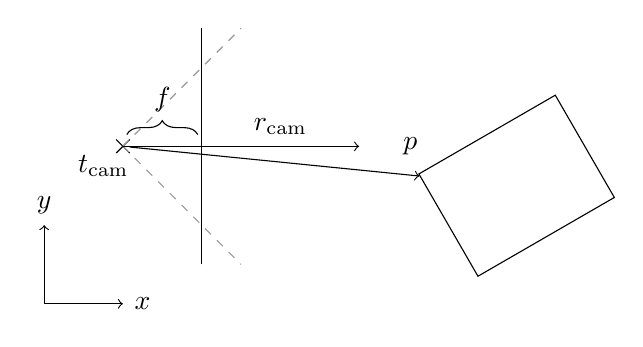
\begin{tikzpicture}
      \node[cross] (c) at (0,0) {};
      \node at (-0.25,-0.25) {$t_{\text{cam}}$};
      
      \draw[-] (1,-1.5) -- (1,1.5);
      %\draw[-] (0,0) -- (0.5,0.5);
      \draw[-,dashed,draw=black!40] (0,0) -- (1.5,1.5);
      %\draw[-] (0,0) -- (0.5,-0.5);
      \draw[-,dashed,draw=black!40] (0,0) -- (1.5,-1.5);
      %\draw[-] (0.5,0.5) -- (0.5,-0.5);
      
      \draw[->] (0,0) -- (3,0);
      \node[] at (2,0.25) {$r_{\text{cam}}$};
      
      \draw [decorate,decoration={brace,amplitude=5pt}]
  (0.05,0.15) -- (0.95,0.15);
      \node at (0.5, 0.6) {$f$};

      \draw[->] (-1,-2) -- (-1,-1) node at (-1,-0.75) {$y$};
      \draw[->] (-1,-2) -- (0,-2) node at (0.25,-2) {$x$};
      
      \node[minimum width=2cm,minimum height=1.5cm,rotate=30,draw=black,rectangle] (r) at (5,-0.5){};
      
      \draw[->] (c) -- (r);
      \node at (3.65,0) {$p$};
  \end{tikzpicture}
\end{figure}
\end{document}